\documentclass{article}
\usepackage{amsmath}
\usepackage{amssymb}
\usepackage{tikz}
\usepackage{array}

\begin{document}

\title{Method 5 - Pandoc Pipeline Test Document - Simple Version}
\maketitle

\section{Mathematical Content}
The quadratic formula is $x = \frac{-b \pm \sqrt{b^2 - 4ac}}{2a}$

\begin{align}
E &= mc^2\\
F &= ma\\
\nabla \times \vec{E} &= -\frac{\partial \vec{B}}{\partial t}
\end{align}

\section{TikZ Graphics}
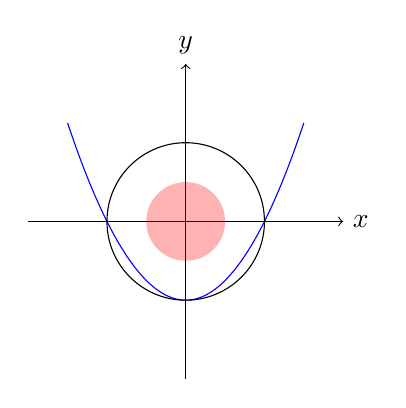
\begin{tikzpicture}
\draw[->] (-2,0) -- (2,0) node[right] {$x$};
\draw[->] (0,-2) -- (0,2) node[above] {$y$};
\draw[domain=-1.5:1.5,smooth,variable=\x,blue] plot ({\x},{\x*\x-1});
\draw (0,0) circle (1cm);
\draw (0,0) -- (1,0);
\draw (0,0) -- (0,1);
\fill[red,opacity=0.3] (0,0) circle (0.5cm);
\end{tikzpicture}

\section{Additional TikZ - Scope Environment}
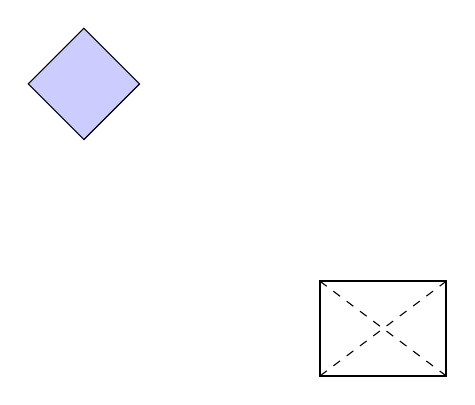
\begin{tikzpicture}
\begin{scope}[shift={(3,0)}, scale=0.8]
\draw[thick] (0,0) rectangle (2,1.5);
\draw[dashed] (0,0) -- (2,1.5);
\draw[dashed] (0,1.5) -- (2,0);
\end{scope}
\begin{scope}[shift={(0,3)}, rotate=45]
\draw[fill=blue!20] (0,0) -- (1,0) -- (1,1) -- (0,1) -- cycle;
\end{scope}
\end{tikzpicture}

\section{Tabular Data}
\begin{table}[h]
\centering
\begin{tabular}{|c|c|c|}
\hline
Method & Speed & Quality \\
\hline
pdflatex & Fast & Good \\
xelatex & Medium & Excellent \\
lualatex & Medium & Very Good \\
\hline
\end{tabular}
\caption{Comparison of LaTeX engines}
\end{table}

\section{Additional Table}
\begin{table}[h]
\centering
\begin{tabular}{|l|r|r|}
\hline
Package & Lines & Complexity \\
\hline
amsmath & 2000+ & Medium \\
tikz & 50000+ & High \\
array & 500+ & Low \\
\hline
\end{tabular}
\caption{Package statistics}
\end{table}

\section{Mathematical Examples}
Some inline math: $\int_0^\infty e^{-x^2} dx = \frac{\sqrt{\pi}}{2}$

Display math:
\begin{equation}
\sum_{n=1}^\infty \frac{1}{n^2} = \frac{\pi^2}{6}
\end{equation}

Matrix example:
\begin{equation}
\begin{pmatrix}
a & b \\
c & d
\end{pmatrix}
\begin{pmatrix}
x \\
y
\end{pmatrix}
=
\begin{pmatrix}
ax + by \\
cx + dy
\end{pmatrix}
\end{equation}

\end{document}
